\chapter{Basic}

%%%%%%%%%%%%%%%%%%%%%%%%%%%%%%%%%%%%%%%%%%%%%%%%%%%%%%%%%%%%%%%%%%%%%%%%
% Document classes
\section{Document classes}
\begin{description}[style=nextline]
    \item [article] 
	For articles in scientific journals, presentation, short
	reports, program documentation, invitations, etc
    \item [report]  
	For longer reports containing several chapters, small
	books, thesis, etc
    \item [book] 
	For real books
    \item [slides]
	For slides, this class uses big sans serif letters
    \item [letter]
	For letter
    \item [beamer]
	For presentations.
\end{description}
%%%%%%%%%%%%%%%%%%%%%%%%%%%%%%%%%%%%%%%%%%%%%%%%
\subsection{Document Class Options} 
\begin{description}[style=nextline]
    \item [11pt]
	Font size, default 10pt.
    \item [a4paper]
	Paper size, default letterpaper. Available options:
	a5paper, b5paper, executivepaper and legalpaper.
    \item [fleqn]
	Typesets displayed formula left-aligned instead of
	centered(default).
    \item [leqno]
	Places the numbering of formulas on the left hand side
	instead of the right(default).
    \item [titlepage, notitlepage]
	The article class does not start a new
	page by default, while report and book do.
    \item [twocolumn]
	Two columns, default one.
    \item [twoside,oneside]
	The article and report classes are single sides
	and the book class is double sided by default. 
    \item [landscape]
	landscape mode. default portrait.
    \item [openright,openany]
	Begin a chapter either only on right hand
	pages or on the next page available. This does not apply to
	\textit{article} class, as it doesn't know about chapters. The
	report class by default starts chapters on the next page available
	and the book class starts them on right hand pages.
    \item [draft,final]
	draft mode, which will speed up typesetting, because
	figures are not loaded, just indicated by a frame. In draft mode,
	\LaTeX{} indicates hyphenation and justification problems with a
	small square in the right-hand margin of the problem line so they
	can be located quickly.
\end{description}
%%%%%%%%%%%%%%%%%%%%%%%%%%%%%%%%%%%%%%%%%%%%%%%%
\subsection{Papersize}
\begin{description}
    \item [letterpaper]	$11 \times 8.5 $ in
    \item [legalpaper]	$14 \times 8.5 $ in
    \item [executivepaper]  $10.5 \times 7.25 $ in
    \item [a4paper] $20.7 \times 21$ in
    \item [a5paper] $21 \times 14.8$ in
    \item [b5paper] $25 \times 17.6$ in
\end{description}


%%%%%%%%%%%%%%%%%%%%%%%%%%%%%%%%%%%%%%%%%%%%%%%%%%%%%%%%%%%%%%%%%%%%%%%%
\section{Sections}
\LaTeX{} provides 7 levels of depth for defining sections.
\begin{description}[style=nextline]
    \item [part]
	level -1, not in letters.
    \item [chapter] 
	level 0, only books and reports.
    \item [section] 
	level 1, not in letters.
    \item [subsection] 
	level 2, not in letters.
    \item [subsubsection] 
	level 3, not in letters.
    \item [paragraph] 
	level 4, not in letters.
    \item [subparagraph] 
	level 5, not in letters.
\end{description}

%%%%%%%%%%%%%%%%%%%%%%%%%%%%%%%%%%%%%%%%%%%%%%%%
\subsection{Options}
    For some section with very long title, \LaTeX{} arrows you to give an
    optional extra version in the Table of Contents and any running heads.
    For example, \verb|\section[Short Name]{Very long title}|, with this
    command, \textbf{Short Name} will appears in \TOC{}, instead of the Very
    long title. 
% Special Characters 

Each sections command also has a "starred" version which does not produce
numbers. Because the *-form sectioning commands don't enter \TOC{}
automatically, \LaTeX{} offers two commands to insert such info directly
into a contents file: \\
\verb|\addtocontents{file}{text}| or
\verb|\addcontentsline{file}{type}{text}|
\begin{description}
    \item [file]    the extension of the contents file, usually toc, lof or
	lot.
    \item [type]    For \textit{lof} or \textit{lot},  \textit{figure} or
	\textit{table} is specified.
    \item [text]    Actually info written to \TOC{}.
\end{description}

%%%%%%%%%%%%%%%%%%%%%%%%%%%%%%%%%%%%%%%%%%%%%%%%
\subsection{\TOC{}}
One can modify the style of \TOC{}.

%%%%%%%%%%%%%%%%%%%%%%%%%%%%%%%%%%%%%%%%%%%%%%%%%%%%%%%%%%%%%%%%%%%%%%%%
\section{Special Characters and Phrases}
\begin{table}
    \centering
    \caption{Special Characters}
    \label{tab:spe_chars}
    \begin{tabular}{|cl|}
	\hline
	\textasciitilde	& \textbackslash{textasciitilde} or \textbackslash{\~{}\{\}}	\\
	\&  & \textbackslash{}\&    \\
	\#  & \textbackslash{}\#    \\
	\_  & \textbackslash{}\_    \\
	\$  & \textbackslash{}\$    \\
	\textbackslash{}    & \textbackslash{textbackslash} \\
	\%  & \textbackslash{}\%    \\
	\textasciicircum    & \textbackslash{textasciicircum} or \textbackslash{\^{}\{\}}  \\
	\{  & \textbackslash{}\{    \\
	\}  & \textbackslash{}\}    \\
	\hline
	\textless, \textgreater	& \textbackslash{textless}, \textbackslash{textgreater}	\\
	\hline
    \end{tabular}
\end{table}

\begin{description}[style=nextline]
    \item [\LaTeX{}]	\verb|\LaTeX{}| 
    \item [\~{}]	Non breakable space
    \item [\ldots]	\verb|\ldots|
\end{description}

%%%%%%%%%%%%%%%%%%%%%%%%%%%%%%%%%%%%%%%%%%%%%%%%
\subsection{Special Symbols}
\begin{table}
    \centering
    \begin{tabular}{ll}
	\verb|\oe, \OE|	&   \oe, \OE	\\
	\verb|\ae, \AE|	&   \ae, \AE	\\
	\verb|\aa, \AA|	&   \aa, \AA	\\
	\verb|\o, \O|	&   \o, \O	\\
	\verb|\l, \L|	&   \l, \L	\\
	\verb|\ss|	&   \ss	\\
	\verb|?`|	&   ?`	\\
	\verb|!`|	&   !`	\\
	\verb|\dag|	&   \dag	\\
	\verb|\ddag|	&   \ddag	\\
	\verb|\S|	&   \S	\\
	\verb|\P|	&   \P	\\
	\verb|\copyright|   &   \copyright	\\
	\verb|{\it \$}|	&   {\it \$}	\\
	\verb|{\it \&}|	&   {\it \&}	\\
	\verb|\i|	&   \i	\\
	\verb|\j|	&   \j	\\
    \end{tabular}
\end{table}

%%%%%%%%%%%%%%%%%%%%%%%%%%%%%%%%%%%%%%%%%%%%%%%%
\subsection{Space}
option to \verb|\\| like this \verb|\\[10pt]|	\\[10pt]
change the vertical distance between lines. \\
Horizontal space \verb|\hspace{1cm}|


Vertical space:	\\
This is \verb|\smallskip| 
\smallskip 
This is \verb|\medskip| 
\medskip
This is \verb|\bigskip|
\bigskip
End

%%%%%%%%%%%%%%%%%%%%%%%%%%%%%%%%%%%%%%%%%%%%%%%%
\subsection{Dashes}
\begin{description}
    \item[-]	hyphen 'double-quote'
    \item[-{}-]	dash denoting a range, e.g. 155--159
    \item[-{}-{}-]	punctuation dash---here it is.
\end{description}

%%%%%%%%%%%%%%%%%%%%%%%%%%%%%%%%%%%%%%%%%%%%%%%%
\subsection{Accents}
There are a variety of control sequences for producing accents.
\begin{table}
    \centering
    \begin{tabular}{ccc}
	{\bf accent}	& {\bf command}	& {\bf example}	\\
	acute	& \verb|\'{a}|	&   \'{a}   \\
	grave	& \verb|\`{a}|	&   \`{a}   \\
	umlaut	& \verb|\"{a}|	&   \"{a}   \\
		& \verb|\={a}|	&   \={a}  \\
		& \verb|\^{a}|	&   \^{a}   \\
		& \verb|\"{a}|	&   \"{a}   \\
		& \verb|\~{a}|	&   \~{a}   \\
		& \verb|\.{a}|	&   \.{a}   \\
		& \verb|\u{a}|	&   \u{a}   \\
		& \verb|\v{a}|	&   \v{a}   \\
		& \verb|\H{a}|	&   \H{a}   \\
		& \verb|\t{aa}|	&   \t{aa}   \\
		& \verb|\c{a}|	&   \c{a}   \\
		& \verb|\d{a}|	&   \d{a}   \\
		& \verb|\b{a}|	&   \b{a}   \\
    \end{tabular}
\end{table}
These accents {\bf cannot} be used within mathematical formulae, some
different control sequencys are used to produce accents within mathematics.

%%%%%%%%%%%%%%%%%%%%%%%%%%%%%%%%%%%%%%%%%%%%%%%%%%%%%%%%%%%%%%%%%%%%%%%%
\section{Alignment}
Command \verb|\begin{center} ... \end{center}| and \\
\verb|\begin{flushright} ... \end{flushright}| and \\
\verb|\begin{flushleft} ... \end{flushleft}| \\
to align in center, right and left

%%%%%%%%%%%%%%%%%%%%%%%%%%%%%%%%%%%%%%%%%%%%%%%%%%%%%%%%%%%%%%%%%%%%%%%%
\section{Font}
The default font used by Palin TeX is \textbf{cmr10}, Knuth only put 128 
glyphs in the fonts, and the char encoding is somewhat different from 
ASCII. So to play chars not in cmr10, you have to specify the texttype,
for example:
\verb|{\tt\string\TeX}|

%%%%%%%%%%%%%%%%%%%%%%%%%%%%%%%%%%%%%%%%%%%%%%%%
\subsection{{\it italic correction}}
\begin{lstlisting}[language=TeX]
{\it italicized\/} or {\sl slanting type\/} correction.
\end{lstlisting}
The control command \verb|\/| produces the so-called {\it italic correction}, 
which is recommended when changing font back from an {\it italic} or 
{\sl slanted} into a {\rm roman} or {\bf boldface} font, in order to produce
extra space to compensate for the way in which some {\it italic} and 
{\sl slanted} letters lean into the following blank space. However, this
italic correction should not be used before a comma or a full stop.

%%%%%%%%%%%%%%%%%%%%%%%%%%%%%%%%%%%%%%%%%%%%%%%%
\subsection{Families}
By default, \LaTeX{} use serif typeface(roman) font. Other font typefaces
(sans serif, typewriter, a.k.a monospace) can be used with some specific 
commands.
\textrm{serif(roman) family}	\\
\textsf{sans serif family}      \\
\texttt{typewriter(monospace) family}	\\
\ttfamily
switch to ttfamily  \\
\sffamily
switch to sffamily  \\
\rmfamily
switch back to default one. \\

To change the default fonts, use the commands:	\\
\command|\renewcommand{\familydefault}{\sfdefault}|

%%%%%%%%%%%%%%%%%%%%%%%%%%%%%%%%%%%%%%%%%%%%%%%%
\subsection{Style}
\textmd{medium};    \\
\textbf{bold}; \\
\textup{upright};   \\
\textsl{slanted style, which makes the text look a bit like \textit{italics}
but not quite}; \\
\textsc{small caps}. \\
\underline{underline}	\\
The corresponding switch commands are:
\begin{lstlisting}[language=TeX]
\mdseries
\bfseries
\upshape 
\itshape or \it
\slshape or \sl
\scshape or \sc
\end{lstlisting}
If you look closely, you will notice that italic text is not only slanted
but that different letters are actually used (e.g. a and {\it a}). 
However, this is only true for serif text, not for sans-serif text. Text
that is only slanted without using different characters is called 
``slanted'' instead of ``italic''.

%%%%%%%%%%%%%%%%%%%%%%%%%%%%%%%%%%%%%%%%%%%%%%%%
\subsection{Size}
{\Huge Huge} \\
{\huge huge} \\
{\LARGE LARGE}	\\
{\Large Large}	\\
{\large large}	\\
{\small small}	\\
{\footnotesize footnotesize} \\
{\scriptsize scriptsize}	\\
{\tiny tiny} \\
{\normalsize normalsize (default)}    \\
All the sizes of other commands depends on the size of normal text.


%%%%%%%%%%%%%%%%%%%%%%%%%%%%%%%%%%%%%%%%%%%%%%%%%%%%%%%%%%%%%%%%%%%%%%%%
\section{Color}
To color text in \LaTeX{}, use \package{xcolor} package. There are 
two syntax to add color to text:
\begin{lstlisting}[language=TeX]
\colorbox{color}{text}	% background color
\textcolor{color}{text}	% text color
{\color{color} some text}
\textcolor{color!20!}{text}	% use 20% of choosed color
\end{lstlisting}
\red{red}, \green{green}, \blue{blue}.
\colorbox{blue!30}{blue}

\newpage
% \pagecolor{gray!50!}   % background
% \color{blue}	% text 
%%%%%%%%%%%%%%%%%%%%%%%%%%%%%%%%%%%%%%%%%%%%%%%%
\subsection{pagecolor}
Use command \verb|\pagecolor{colorg}| to set the background color of page.

{\color{red} For unknown reason, if I change the bg color with 
\verb|\pagecolor{color}|, the `Go to TOC' button will fail in the 
following pages (including the current one).}
% \lipsum[1-3]
\newpage
% \pagecolor{white} \color{black}

%%%%%%%%%%%%%%%%%%%%%%%%%%%%%%%%%%%%%%%%%%%%%%%%
\subsection{Basic colors names available in \LaTeX{}}
black, blue, brown, cyan, darkgray, gray, green, lightgray, lime, 
magenta, olive, orange, pink, purple, red, teal, violet, white, yellow.
% \box

%%%%%%%%%%%%%%%%%%%%%%%%%%%%%%%%%%%%%%%%%%%%%%%%%%%%%%%%%%%%%%%%%%%%%%%%
\section{Footer and Header}
Use command \verb|\pagestyle{style}| or \verb|\thispagestyle{style}| 
to set page style, the possible styles are:
\begin{description}[style=nextline]
    \item [plain]   default style. The header is empty and the footer
	contains page numbers in the center.
    \item [empty]   Both header and footer are cleared.  
    \item [headings]	Puts running headings on each page. The document
	style specifies what goes in the headings.
    \item [myheadings]	You specify what is to go in the heading with the
	\verb|\markboth| or the \verb|\markright| commands. 
	The footer is empty in this page style. The header
	contains the page number on right side (on even pages) or on left
	side (on odd pages) along with other user-supplied information;
	there is an exception for the first page of each chapter, where the
	footer contains centred page number while the header is blank.
\end{description}

\thispagestyle{fancy}   % set fancy style
\fancyhf{}  % reset current configuration
% the width of the horizonal line between head and contents.
\renewcommand{\headrulewidth}{2pt}
\renewcommand{\footrulewidth}{1pt}
% set header
\rhead{\leftmark}   
\lhead{\rightmark}  
\chead{\thepage}
\rfoot{\thepage}
\lfoot{left foot}
\cfoot{center foot}

For double-sided documents (books), use different command \verb|\fancyhead|
and \verb|fancyfoot| with several options.
\begin{lstlisting}[language=TeX]
\pagestyle{fancy}
\fancyhf{}
% show chapter name in the left of even pages and right of odd pages
\fancyhead[LE,RO] {\leftmark} 
% show section name in the right of even pages and left of odd pages
\fancyhead[RE,LO] {\rightmark} 
% show page number in foot center of even and odd pages
\fancyfoot[CE,CO] {\thepage}	
\end{lstlisting}

%\pagestyle{empty}


% set plain style attribute
% \fancypagestyle{plain} 

This is a footnote \footnote[1]{first footnote} \footnote[2]{second footnote}

The following commands can be used in the headers and footers:
\begin{description}[style=nextline]
    \item [\textbackslash{thepage}] Number of current page
    \item [\textbackslash{thechapter}] Number of current chapter
    \item [\textbackslash{thesection}] Number of current section
    \item [\textbackslash{chaptername}] chapter name
    \item [\textbackslash{leftmark}] Names and number of current top-level
	structure(e.g. \textit{Chapter for reports, Sectoin for articles})
	in uppercase letters.
    \item [\textbackslash{rightmark}] Names and number of current next to 
	top-level structure in uppercase letters.
\end{description}

%%%%%%%%%%%%%%%%%%%%%%%%%%%%%%%%%%%%%%%%%%%%%%%%
\subsection{Pagenumber}
\verb|\pagenumbering{...}|
\begin{description}
    \item [arabic]
    \item [roman]   lowercase
    \item [Roman]   Uppercase
    \item [alph]    lowercase English letters
    \item [Alph]    Uppercase
\end{description}

%%%%%%%%%%%%%%%%%%%%%%%%%%%%%%%%%%%%%%%%%%%%%%%%%%%%%%%%%%%%%%%%%%%%%%%%
\section{Length}

\subsection{Unit}
\begin{description}
    \item [\textbf{sp}] scaled point,  65535 sp = 1 pt
    \item [\textbf{pt}]	point, 1/72.27 in, or 0.0138 in or 0.3515 mm
    \item [\textbf{bp}] big point,  1 in = 72 bp
    \item [\textbf{dd}] didot point,  1157 dd = 1238 pt
    \item [\textbf{mm}] a millimeter
    \item [\textbf{pc}] pica,  1 pc = 12 pt = 4.218 mm
    \item [\textbf{cc}] cicero,  1 cc = 12 dd = 4.513 mm
    \item [\textbf{cm}] a centimeter
    \item [\textbf{in}] a inch = 25.4 mm
    \item [\textbf{ex}] roughtly the height of an `x' (lowercase) in the current \textbf{font}
    \item [\textbf{em}] roughtly the width of an `M' (Uppercase) in the current \textbf{font}
    \item [\textbf{mu}] math unit = 1/18 em, where \textbf{em} is taken from the math 
	symbols family.
\end{description}
Hou much a point is depends on whom you ask. \TeX{} thinks a point is the
72.27th part of an inch, which is 2.54 cm. On the other hand, PostScript
and Adobe think a point is the 72th part of an inch (which is a big point
in \TeX{}).

%%%%%%%%%%%%%%%%%%%%%%%%%%%%%%%%%%%%%%%%%%%%%%%%
\subsection{general length}
\begin{table}[htb]
    \centering 
    \begin{tabular}{cc}
	\verb|\hskip| {\it length}  & horitontal blank space of {\it length}	\\
	\verb|\vskip| {\it length}  & vertical blank space of {\it length}	\\
    \end{tabular}
\end{table}

Note: If the word following the horizontal skip happens to be \lq plus \rq then 
you will probably get an error message:
\begin{lstlisting}[language=TeX]
    ! Missing number, treated as zero.
\end{lstlisting}
To avoid it, typing `\verb|\hskip 20 mm \relax|'

%%%%%%%%%%%%%%%%%%%%%%%%%%%%%%%%%%%%%%%%%%%%%%%%
\subsection{Structured length}
\begin{description}
    \item [\textbackslash{}baselineskip]    Vertical distance between lines in a paragraph.
    \item [\textbackslash{}columnsep]	    column separation
    \item [\textbackslash{}columnwidth]	    the width of a column
    \item [\textbackslash{}evensidemargin]  
    \item [\textbackslash{}oddsidemargin]    
    \item [\textbackslash{}linewidth]    
    \item [\textbackslash{}lineskip]    
    \item [\textbackslash{}paperwidth]    
    \item [\textbackslash{}paperheight]    
    \item [\textbackslash{}parskip]	    Vertical space between paragraphs
    \item [\textbackslash{}tabcolsep]    
    \item [\textbackslash{}textheight]	    Height of the text area in the page
    \item [\textbackslash{}textwidth]    
    \item [\textbackslash{}topmargin]    
\end{description}
%%%%%%%%%%%%%%%%%%%%%%%%%%%%%%%%%%%%%%%%%%%%%%%%
\subsection{table}
Length between columns :
\verb|\setlength{\tabcolsep}|	

%%%%%%%%%%%%%%%%%%%%%%%%%%%%%%%%%%%%%%%%%%%%%%%%%%%%%%%%%%%%%%%%%%%%%%%%
\section{Space}
First note that, as a general rule, you should never put a blank space after
a left parenthesis or before a right parenthesis. If you were to put a blank
space in these places, then you run the risk that \TeX{} might start a new line
immediately after the left parenthesis or before the right parenthesis, 
leavin the parenthesis marooned at the beginning or end of a line.

\TeX{} has its own rules for deciding the lengths of blank spaces. For instance,
\TeX{} will put an extra amount of space after a full stop if it considers
that the full stop marks the end of a sentence.

The rule adopted by \TeX{} is to regard a period (full stop) as the end of a
sentence if it is preceded by a lowercase letter. If the period is preceded by
an uppercase letter then \TeX{} assumes that it is not a full stop but follows
the initials of somebody's name.

This works very well in most cases. However \TeX{} occasionally gets things
wrong. This happens with a number of common abbreviations (as in `Mr.~Smith' 
or in `etc.'), and, in particular, in the names of journals given in
abbreviated form (e.g., `Proc. Amer. Math. Soc.'). The way to overcome this
problem is to put a backslash before the blank space in question. Thus we
should type:
\begin{lstlisting}[language=TeX]
    Mr.\ Smith
    etc.\ and
    Proc.\ Amer.\ Math.\ Soc.
\end{lstlisting}

\TeX{} determines itself how to break up a paragraph into lines, and will
occasionally hyphenate long words where this is desirable. However it is
sometimes necessary to tell \TeX{} not to break at a particular blank space.
The special character used for this purpose is \textasciitilde. It represents 
a blank space at which \TeX is not allowed to break between lines. It is often 
desirable to use \textasciitilde in names where the forenames are represented 
by initials. Thus to obtain `W.~R.~Hamilton' it is best to type 
W.\textasciitilde R.\textasciitilde Hamilton.

%%%%%%%%%%%%%%%%%%%%%%%%%%%%%%%%%%%%%%%%%%%%%%%%%%%%%%%%%%%%%%%%%%%%%%%%
\section{Commands}

\subsection{newcommand}
\command|\def| can define commands that take delimiters other than braces,
while \command|\newcommand| can't.  \\
\command|\def\foo<#1>{something #1}|	\\
\command|\foo<happy>|

%%%%%%%%%%%%%%%%%%%%%%%%%%%%%%%%%%%%%%%%%%%%%%%%%%%%%%%%%%%%%%%%%%%%%%%%
\section{List}
Three are three kinds of list in \LaTeX{}: 

\subsubsection{itemize}
\begin{itemize}
    \item First item
    \item Another item
\end{itemize}

\subsubsection{enumerate}
\begin{enumerate}
    \item One
    \item Two
\end{enumerate}

\subsubsection{description}
\begin{description}
    \item[Foo] Foo 
    \item[Bar] Bar
    \item[description] \hfill \\
	Use \textbackslash{fill} so that the explanaion begins in newline.
\end{description}

%%%%%%%%%%%%%%%%%%%%%%%%%%%%%%%%%%%%%%%%%%%%%%%%
\subsection{Bullet}
One can change the bullet of a list easily without loading any package.

%%%%%%%%%%%%%%%%%%%%%%%%
\subsubsection{Unordered lists}
\begin{itemize}
    \item[--] dash
    \item[$\ast$] asterisk
    \item[$\alpha$] Any math character
    \item[a] Char
\end{itemize}

%%%%%%%%%%%%%%%%%%%%%%%%
\subsubsection{Ordered lists}

roman:	\\
\begin{enumerate}[label = (\roman*)]	% this option require enumitem package
    \item enumerate
    \item Option (A1) specify label 'A'.
\end{enumerate}

Roman:
\begin{enumerate}[label=(\Roman*)]
    \item One
    \item Two
\end{enumerate}

arabic:
\begin{enumerate}[label = (\arabic*)]
    \item One
    \item Two
\end{enumerate}

alph:
\begin{enumerate}[label = (\alph*)]
    \item a
    \item b
\end{enumerate}

Alph:
\begin{enumerate}[label = (\Alph*)]
    \item a
    \item b
\end{enumerate}

%%%%%%%%%%%%%%%%%%%%%%%%%%%%%%%%%%%%%%%%%%%%%%%%%%%%%%%%%%%%%%%%%%%%%%%%
\section{Table}

\verb|\toprule, \midrule, \bottomrule| used as seperation line.

%%%%%%%%%%%%%%%%%%%%%%%%%%%%%%%%%%%%%%%%%%%%%%%%
\subsection{tabbing}
\emph{tabbing} env. can also produce table format:
\begin{tabbing}
    \textbf{AbiWord}\quad\= : \= A word processor\kill \\
    \textbf{\TeX}\quad	 \> : \> A typesetting program \\[5pt]
    \textbf{Emacs}\quad	 \> : \> A text editor \\[5pt]
			 \>   \> \quad\= a programming env. \\[5pt]
			 \>   \>      \> a mail reader \\[5pt]
			 \>   \>      \> and a lot more besides \\[5pt]
    \textbf{AbiWord}\quad\> : \> A word processor
\end{tabbing}

The alighment of text can be: l,c,r or p{length}

\begin{center}
    \begin{tabular}{lp{6cm}}
	Planet	& Features\tabularnewline[8pt]
	Mercury	& \raggedright	Lunar like crust \\
				Crustal faulting \\
				Small magnetic fiels\tabularnewline[3pt]
		& Guess what's this \\
    \end{tabular}
\end{center}

%%%%%%%%%%%%%%%%%%%%%%%%%%%%%%%%%%%%%%%%%%%%%%%%
\subsection{Multi-columns or rows}
\verb|multicolumn{num}{pos}{item}|
\begin{center}
    \begin{tabular}{|l|r|r|}
	\hline
	Planet	& \multicolumn{2}{c|}{Distance from sum (km)}\\
	\cline{2-3} 
		& Maximum   & Minimum   \\
	\hline
	Mercury	& 69400000  & 46800000	\\
	Pluto	& 734600000 & 4461000000    \\
	\hline
    \end{tabular}
\end{center}
Similarly, we can apply 
\command|\multirow[pos]{num}{*}{item}| when include
\package{multirow} package.

\begin{center}
    \begin{tabular}{|l|r|r|}
	\hline
		& \multicolumn{2}{p{3.5cm}|}{\centering Distance from sum
	        \\ (kilometer)}\\
	\cline{2-3} 
	\multicolumn{1}{|c|}{Planet}	& \multicolumn{1}{c|}{Maximum}	
		& \multicolumn{1}{c|}{Minimum}   \\
	\hline
	Mercury	& 69400000  & 46800000	\\
	Pluto	& 734600000 & 4461000000    \\
	\hline
    \end{tabular}
\end{center}

\begin{center}
    \begin{tabular}{|c|r@{--}l|}
	\hline
	Height	& \multicolumn{2}{c|}{Ideal weight} \\
	(cm)	& \multicolumn{2}{c|}{(kg)} \\
	\hline
	155 & 53.5  & 64    \\
	160 & 56    & 67    \\
	190 & 78    & 92.5  \\
	\hline
    \end{tabular}
\end{center}

%%%%%%%%%%%%%%%%%%%%%%%%%%%%%%%%%%%%%%%%%%%%%%%%
\subsection{Colors}
To setup row and column color, use package:
\package{\textbackslash{}usepackage[table]\{xcolor\}}

\definecolor{lightgray}{gray}{0.9}
%%%%%%%%%%%%%%%%%%%%%%%%
\subsubsection{Single row or column and single cell}
\begin{center}
    \rowcolors{1}{}{lightgray}	% change color in odd and pair rows
    \begin{tabular}{| l | c |}
	\hline
	J.\ S.\ Bach	& 1685--1750	\\
	\rowcolor{lightgray}
	W.\ A.\ Mozart	& 1756--1791	\\
	L.\ Beethoven	& 1770--1827	\\
	\hline
    \end{tabular}
\end{center}

\newcolumntype{r}{>{\columncolor{red}}c}
\newcolumntype{g}{>{\columncolor{green}}c}
\newcommand{\ra}{\rand0.\arabic{rand}}
\begin{table}[ht]
    \centering
    \begin{tabular}{c | r | c | g | c | >{\columncolor{blue}}c | c}
    \hline
	& col1	& col2	& col3	& col4	& col5	& col6	\\
    \hline
    row1 & \ra & \ra & \ra & \ra & \ra & \ra \\
    row2 & \ra & \ra & \ra & \ra & \ra & \ra \\
    row3 & \ra & \ra & \ra & \ra & \ra & \ra \\
    row4 & \ra & \ra & \ra & \ra & \ra & \ra \\
    \hline
    \end{tabular}
\end{table}

\begin{center}
    \begin{tabular}{ | l | l | l | }
      \hline
      A & B & C \\
      \hline
      D & E & \cellcolor{green}F \\
      \hline
      G & H & I \\
      \hline
    \end{tabular}
\end{center}

%%%%%%%%%%%%%%%%%%%%%%%%
\subsubsection{Alternating row}
\begin{center}
    \rowcolors{1}{}{lightgray}	% change color in odd and pair rows
    \begin{tabular}{| l | c |}
	\hline
	J.\ S.\ Bach	& 1685--1750	\\
	W.\ A.\ Mozart	& 1756--1791	\\
	L.\ Beethoven	& 1770--1827	\\
	F.\ Chopin	& 1810--1849	\\
	R.\ Schumann	& 1810--1856	\\
	B.\ Bartok	& 1881--1945	\\
	\hline
    \end{tabular}
\end{center}

%%%%%%%%%%%%%%%%%%%%%%%%
\subsubsection{multirow or multicol}
When use \command|\rowcolor| in \command|\multirow|
or \command|\multicolumn| environment, if it is not put at the start
of a new line, it will raise a \error{Misplace noalign}. You can either ignore it or you can use \command|\cellcolor| from the same package.

\begin{table}[ht]
    \rowcolors{1}{}{lightgray}
    \centering
    \caption{Multirow table with all cells in the same color.}
    \label{tab:multi row}
    \begin{tabular}{p{5cm}p{5cm}}
	\hline
	Column 1 & Column 2\\
	\hline
	-&-\\
	-&-\\
	\cellcolor{lightgray}&Single-row\\
	\cellcolor{lightgray}&Single-row\\
	\multirow{-3}{*}{\cellcolor{lightgray}Multi-row (3)}	& Single-row	\\
	-&-\\
	-&-\\
	\hline
    \end{tabular}
\end{table}%


%%%%%%%%%%%%%%%%%%%%%%%%
\subsubsection{Line color}
use command \command|\arrayrulecolor{color}|:

\arrayrulecolor{blue}

\begin{center}
    \begin{tabular}{ | l | l | l | }
      \hline
      A & B & C \\
      \hline
      D & E & F\\
      \hline
      G & H & I \\
      \hline
    \end{tabular}
\end{center}
%%%%%%%%%%%%%%%%%%%%%%%%%%%%%%%%%%%%%%%%%%%%%%%%
\subsection{alignment}
Using package \package{tabularx}, one can manipulate the alignment of the
cells.

flush left fixed width:
\verb|\newcolumntype{L}[1]{>{\raggedright\arraybackslash}p{#1}}|

center fixed width:
\verb|\newcolumntype{C}[1]{>{\centering\arraybackslash}p{#1}}|

flush right fixed width:
\verb|\newcolumntype{R}[1]{>{\raggedleft\arraybackslash}p{#1}}|

\newcolumntype{L}[1]{>{\raggedright\arraybackslash}p{#1}}
\newcolumntype{C}[1]{>{\centering\arraybackslash}p{#1}}
\newcolumntype{R}[1]{>{\raggedleft\arraybackslash}p{#1}}

\begin{tabular}{|L{1cm}|C{2cm}|R{3cm}|}
    \hline
    1cm width	& 2cm width & 3cm width	\\
    \hline
    left    & center	& right	\\
    \hline
\end{tabular}

%%%%%%%%%%%%%%%%%%%%%%%%%%%%%%%%%%%%%%%%%%%%%%%%
\subsection{centering a wide table}
To center a very wide table, you can take the following ways:
\begin{itemize}
    \item \verb|\makebox[\textwidth][c]{<table>}|
    \item use adjustbox (from package \package{adjustbox})
	\begin{verbatim}
	\begin{adjustbox}{center}
	    \begin{tabular}{ccc}
		table content
	    \end{tabular}
	\end{adjustbox}
	\end{verbatim}
    \item \verb|\centerline{<table>}|
\end{itemize}



%%%%%%%%%%%%%%%%%%%%%%%%%%%%%%%%%%%%%%%%%%%%%%%%
\subsection{Line height}
\command|\renewcommand{\arraystretch}{2}| to increase the row height to 
2 times of original one. Don't forget to change it back to original value
with \command|\renewcommand{\arraystretch}{1}|. 

To change only height of one row, you can use \command|\rule{0pt}{height} | in the start of a row. 

This trick also change the height of a row by adding extra space to it: 
\command|\\[distance]|. For example: \
command|\\[-1em]|. \command|\\|: add one line of space, 
\command|[\-1em]|: minus 1em from previous spacing.

%%%%%%%%%%%%%%%%%%%%%%%%%%%%%%%%%%%%%%%%%%%%%%%%
\subsection{Line break in a table cell}

\subsubsection{makecell}
Using the \command|\thead| and \command|\makecell| command from package \package{makecell}

\renewcommand\theadalign{bc}
\renewcommand\theadfont{\bfseries}
\renewcommand\theadgape{\Gape[4pt]}
\renewcommand\cellgape{\Gape[4pt]}

\begin{center}
    \begin{tabular}{ | c | c | c |}
	\hline
	\thead{A Head}	& \thead{A Second \\ Head}  & \thead{A Third \\ Head}	\\
	\hline
	Some text   & \makecell{Some really \\ long text}   & \makecell{Another \\ long text}	\\
	\hline
    \end{tabular}
\end{center}

\subsubsection{tabularx}
Use the \emph{tabularx} environment instead of \emph{tabular} from package \package{tabularx}
\begin{center}
    \begin{tabularx}{\textwidth}{lX}
	Section:    & This is my \newline 
		      long paragraph	\\
    \end{tabularx}
\end{center}


%%%%%%%%%%%%%%%%%%%%%%%%%%%%%%%%%%%%%%%%%%%%%%%%
\subsection{Wide table}
use package \package{adjustbox} to fit the width of your table to pages.

\begin{adjustbox}{center}
    \large
    \begin{tabular}{|l|c|c|c|c|c|c|c|c|c|c|c|c|c|}
	\hline
	Name    & lab 1 & lab 2 & lab 3 & lab 4 & lab 5 & lab 6 & lab 7 & lab 8 & lab 9 & lab 10 & lab 11 & lab 12 & lab 13    \\
	\hline
    \end{tabular}
\end{adjustbox}



%%%%%%%%%%%%%%%%%%%%%%%%%%%%%%%%%%%%%%%%%%%%%%%%%%%%%%%%%%%%%%%%%%%%%%%%
\section{Figure}

%%%%%%%%%%%%%%%%%%%%%%%%%%%%%%%%%%%%%%%%%%%%%%%%
\subsection{wrapfig}
Surrounding figures with text using package \package{wrapfig}. Note
that text can't follow the wrapfig env. directly.

\begin{wrapfigure}{L}{0.3\textwidth}
    \centering 
    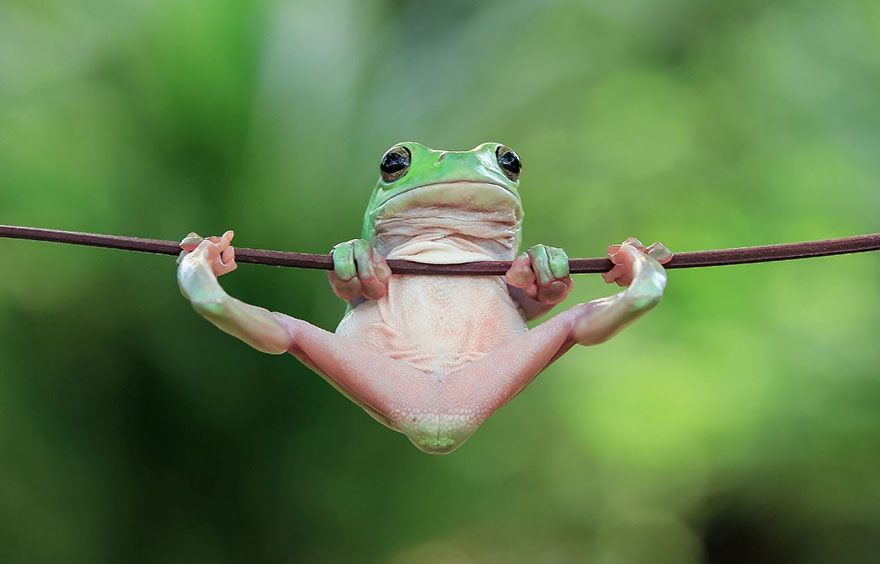
\includegraphics[width=0.25\textwidth]{frog}
    \caption{\label{fig:frog}A frog}
\end{wrapfigure}
% note the blank line here. text can't follow the wrapfig environment directly.

\lipsum[1]

\begin{wrapfigure}{R}{0.3\textwidth}
    \centering 
    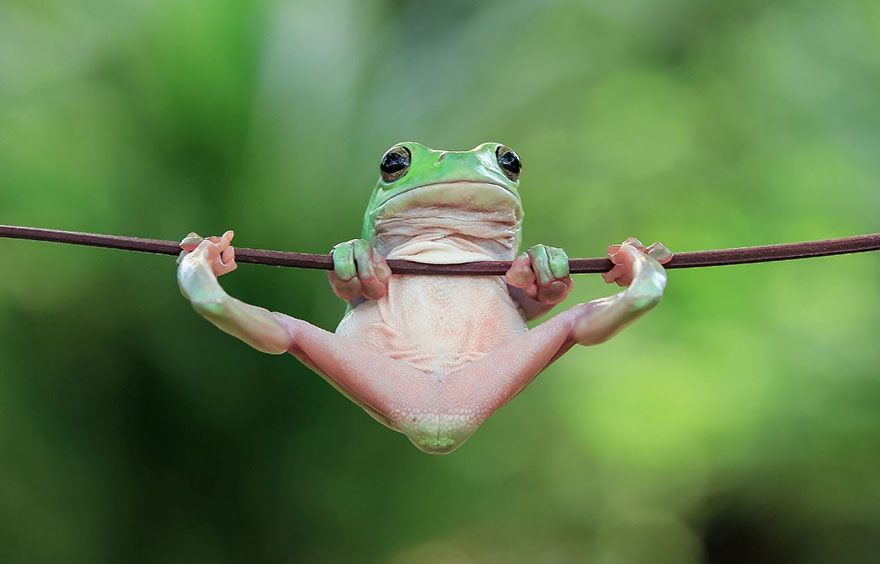
\includegraphics[width=0.25\textwidth]{frog}
    \caption{\label{fig:frog}A frog}
\end{wrapfigure}

\lipsum[2]


%%%%%%%%%%%%%%%%%%%%%%%%%%%%%%%%%%%%%%%%%%%%%%%%
\subsection{minipage}
To use \emph{minipage} environment, note that add a \% behind every 
\verb|\end{minipage}| statement.
\begin{lstlisting}[language=TeX]
    \begin{figure}
	\begin{minipage}{0.5\textwidth}
	\end{minipage}%
	\begin{minipage}{0.5\textwidth}
	\end{minipage}
    \end{figure}
\end{lstlisting}
%%%%%%%%%%%%%%%%%%%%%%%%%%%%%%%%%%%%%%%%%%%%%%%%%%%%%%%%%%%%%%%%%%%%%%%%
\section{Equation}

%%%%%%%%%%%%%%%%%%%%%%%%%%%%%%%%%%%%%%%%%%%%%%%%%%%%%%%%%%%%%%%%%%%%%%%%
\section{Code}

%%%%%%%%%%%%%%%%%%%%%%%%%%%%%%%%%%%%%%%%%%%%%%%%
\subsection{Verbatim}
The default tool to display code in \LaTeX{} is \textbf{verbatim}, which
generates an output in monospaced font. 
\begin{verbatim}
Tex enclodes inside \texttt{verbatim} envi. is printed directl and all
\LaTeX{} commands are ignored.
\end{verbatim}

A starred version of verbatim envi. will produce slightly different output
where white spaces are emphasized with a special symbol.
\begin{verbatim*}
Tex enclodes inside \texttt{verbatim} envi. is printed directl and all
\LaTeX{} commands are ignored.
\end{verbatim*}

Verbatim-like text can also be used in paragraph by means of the
\verb|\verb| command. Any charactre, except letters and *, can be used as
delimiter. For instance \verb+Delimiter+ use + as delimiter.

%%%%%%%%%%%%%%%%%%%%%%%%%%%%%%%%%%%%%%%%%%%%%%%%
\subsection{Highlighting code}
To produce highlight code, we need \package{listings}
\begin{lstlisting}[language=Python]
    import numpy as np

    def f(x1, x2):
	if x1 > x2:
	    print "Hello World"

    a=4, b=5
    f(b, a)
\end{lstlisting}

%%%%%%%%%%%%%%%%%%%%%%%%%%%%%%%%%%%%%%%%%%%%%%%%
\subsection{Importing code from a file}
To import code from files, using command \verb|\lstinputlisting|.
\begin{lstlisting}[language=TeX]
\lstinputlisting[language=Python]{hello_wrold.py}
\lstinputlisting[language=Python, caption = Python]{hello_wrold.py}
\lstinputlisting[language=Python, firstline=2, lastline=12]{hello_wrold.py}
\end{lstlisting}

%%%%%%%%%%%%%%%%%%%%%%%%%%%%%%%%%%%%%%%%%%%%%%%%
\subsection{Code Style}
\package{listings} is highly customisable.  
\begin{lstlisting}[language=TeX]
\definecolor{codegreen}{rgb}{0,0.6,0}
\definecolor{codegray}{rgb}{0.5,0.5,0.5}
\definecolor{codepurple}{rgb}{0.58,0,0.82}
\definecolor{backcolour}{rgb}{0.95,0.95,0.92}

\lstdefinestyle{mystyle}{
    backgroundcolor=\color{backcolour},   
    commentstyle=\color{codegreen},
    keywordstyle=\color{magenta},
    numberstyle=\tiny\color{codegray},
    stringstyle=\color{codepurple},
    basicstyle=\footnotesize,
    breakatwhitespace=false,         
    breaklines=true,                 
    captionpos=b,                    
    keepspaces=true,                 
    numbers=left,                    
    numbersep=5pt,                  
    showspaces=false,                
    showstringspaces=false,
    showtabs=false,                  
    tabsize=2
}

\lstset{style=mystyle}
\end{lstlisting}

%%%%%%%%%%%%%%%%%%%%%%%%%%%%%%%%%%%%%%%%%%%%%%%%
\subsection{listings}

\subsubsection{lstinline}
To wrap \command|lstinline|, one need to avoid to read the argument with
the wrapper macro. Currently, I can't find any method to add background
to inline code using \command|\lstinline|. We have no way to wrap 
\command|\lstinline| in other environments, like \command|\colorbox|
to make background color for it. Even the following fails compilation:	\\
\command|\newcommand{\command}{\lstinline[language=TeX, basicstyle=\color{RawSienna}]}|	\\
\command|\colorbox{gray}{\command#\color#}|

\command|\newcommand\codeinline{\lstinline[style=inlinecode]}|	\\
\command|\codeinline+&$%+|  




%%%%%%%%%%%%%%%%%%%%%%%%%%%%%%%%%%%%%%%%%%%%%%%%%%%%%%%%%%%%%%%%%%%%%%%%
\section{Box}
Use \verb|\makebox| to fit wide table or figures.

\makebox[\textwidth]{
    \begin{tabular}{cc}
	a very long sentences that will fill up the cell, but it will still be centerized.  & this it the right cell that will exceed the right margin.
    \end{tabular}
}
%%%%%%%%%%%%%%%%%%%%%%%%%%%%%%%%%%%%%%%%%%%%%%%%%%%%%%%%%%%%%%%%%%%%%%%%
\section{Miscellaneous}
\verb|\rule{length}{width}|

{\color{red}	\rule{\linewidth}{0.5mm} }
%%%%%%%%%%%%%%%%%%%%%%%%%%%%%%%%%%%%%%%%%%%%%%%%%%%%%%%%%%%%%%%%%%%%%%%%
\section{Reference}
reference command :
\verb|\cite, \ref, \pageref and \label|
Put \verb|\label| in argument of \verb|\section| for cross-referencing:
\verb|\section{\label{}}|

%%%%%%%%%%%%%%%%%%%%%%%%%%%%%%%%%%%%%%%%%%%%%%%%%%%%%%%%%%%%%%%%%%%%%%%%
\section{Bibliography}
to cite a bibliography, use the \verb|\cite| command. 
Please refer to \cite{wiki} or \cite[option]{wiki}.

%%%%%%%%%%%%%%%%%%%%%%%%%%%%%%%%%%%%%%%%%%%%%%%%
\subsection{BIBTeX}
Another way to cite bibliography is using BIBTeX. \\
BIBTeX style:
\begin{description}
    \item [plain] Entries sorted alphabetically with numeric labels.
    \item [unsrt] Entries printed in order of citation.
    \item [alpha] Use author's name and the year of publication as labels.
    \item [abbrv] compact style, first name, month, and journal names are
	abbrevitated
    \item [acm]	it hse author name in small caps, and numbers as labels.
    \item [apalike] require \package{apalike} package. Entries formatted
	alphabetically, last name first, each entry having a hanging
	indentation and no label.
\end{description}

To run BIBTeX with \LaTeX{}, (\Rom{1})\  one needs to run \LaTeX{} firstly to
generate a list of \textbackslash{}cite references in its auxiliary file
.aux. (\Rom{2})\  Then run BIBTeX to read the auxiliary file, looking up the references
in the database, and write results into .bbl file (formatted according to
the format specified in the .bst style file). (\Rom{3})\  Run \LaTeX{} again to read the
.bbl reference file. (\Rom{4})\  Finally run \LaTeX{} a third time, resolving all
reference. 

\begin{thebibliography}{9}
\bibitem{wiki}
    wikipedia.com.
\end{thebibliography}
